%!TEX root = ../Master Thesis.tex

\chapter{Szenario} % (fold)
\label{cha:szenario}

Für die Master Thesis ist es notwendig, dass ein Szenario existiert, anhand dessen eine Anwendung mit dem MIAV Framework entwickelt werden kann. Da das Framework bisher nur als Modell existiert, muss das Szenario sowohl die Anwendung berücksichtigen als auch die Verwendung des Frameworks. Diese erste Version soll dazu als eine Grundlage dienen, die kontinuierlich weiter entwickelt werden muss.

\section{Rahmen des Szenarios} % (fold)
\label{sec:rahmen_des_szenarios}

Bei dem Szenario handelt es sich um eine Lehrveranstaltung, die \textbf{gleichzeitig} an zwei unterschiedlichen Abteilungen der Fachhochschule Köln stattfindet. Dabei ist aber nicht etwa ein Standort der Sender und der andere entsprechend der Empfänger. Zwischen beiden Standorten herrscht eine bidirektionale Verbindung und Interaktionen sind durch Teilnehmer an beiden Standorten möglich und erwünscht.

% section rahmen_des_szenarios (end)

\section{Beschreibung des Szenario} % (fold)
\label{sec:beschreibung_des_szenario}

An der Fachhochschule Köln - Abteilung Gummersbach findet seit diesem Semester das erste Mal die Veranstaltung "`Medienrezeption"' in einer ganz neuen Form statt. Die Idee die dazu geführt hat ist, verwandte Fachbereiche an der Hochschule auch Standortübergreifend besser zu integrieren. Als Pilotprojekt wurde entschieden, dass die Veranstaltung "`Medienrezeption"' auch von den Studenten des Studiengangs "`Medientechnik"' besucht werden kann. Dieser Studiengang wird am Standort Deutz angeboten. Nun ist die Wahrscheinlichkeit sehr gering, dass die Studenten aus Deutz nach Gummersbach wegen diesem einen Fach fahren, egal wie interessant es auch sein mag. Zudem kommen Koordinationsschwierigkeiten mit dem Stundenplan hinzu. Als Lösung wurde ein einfaches Setup installiert, was eine aktive Teilnahme der Studenten beider Standorte an der Veranstaltung erlaubt:

\begin{itemize}

	\item In jedem Standort sind zwei hochauflösende Webcams installiert, eine die den Dozenten zeigt, eine die das Auditorium zeigt.
	\item In jedem Standort sind zwei Beamer installiert, einen für die Bildinformationen des anderen Standortes und einen für die Folien des Dozenten oder der Studenten.
	\item In jedem Standort ist ein Rechner installiert, über den die Kommunikation realisiert wird.
	\item Die Laptops der Studenten oder des Dozenten werden bei Bedarf an den jeweiligen Kommunikationsrechner angeschlossen, der sämtliche Datenübertragung realisiert.
	\item Die Dozenten erhalten ein eigenes Mikrofon und es stehen 2-3 Mikrofone für die Aufzeichnung der Studenten bereit.
	\item Jeder Standort verfügt über ein Lautsprechersystem.

\end{itemize}

Die Veranstaltung "`Medienrezeption"' findet erfahrungsgemäß im kleinen Kreise statt, da es sich um ein Fach im Masterstudiengang handelt. Etwa 10 Studenten der Medieninformatik besuchen sie. Bei den Medientechnikern wird es nicht als Pflichtfach, sondern als Wahlpflichtfach angeboten, daher nehmen in der Pilotphase nur 5 Studenten aus Deutz teil.

Es wird für dieses Setup keine außergewöhnliche Technik benötigt, was die Umsetzung deutlich vereinfacht. Bei allen Komponenten handelt es sich um "`Consumer"'-Artikel, wie man sie in jedem Elektronikmarkt erhalten kann. Lediglich die Verwendung von zwei Beamern ist etwas kostspieliger. Die gesamte Steuerung und Kommunikation wird durch die Applikation auf den Kommunikationsrechnern geregelt, die auf dem MIAV-Framework basiert. Bei den Rechnern handelt es sich ebenfalls um Standard Hardware.

Die Applikation übernimmt unterschiedliche Aufgaben bei diesem Anwendungsfall, so wir von ihr zum einen das Bild beider Kameras zu übertragen zum anderen auch das Signal der jeweils angeschlossenen Rechner. Zusätzlich wird das Audiosignal der Mikrofone übertragen. Die Darstellung des Computersignals erfolgt dabei synchron zu der Darstellung des Videosignals. Die Lautstärke der Mikrofone wird von der Applikation automatisch so angepasst, dass der aktuelle Sprecher optimal zu hören ist und nur wenig Umgebungsgeräusche übertragen werden.

Was ebenfalls von dem System umgesetzt wird, ist das "`Zeigen"' auf Inhalte, die von den Rechnern der Dozenten oder Studenten kommen. Dies wird einfach dadurch realisiert, dass das komplette Videosignal abgegriffen und übertragen wird. Somit also auch der Mauszeiger. In weiteren Versionen wären hier sicherlich intelligentere Methoden denkbar.

\begin{figure}[htbp]
  \centering
    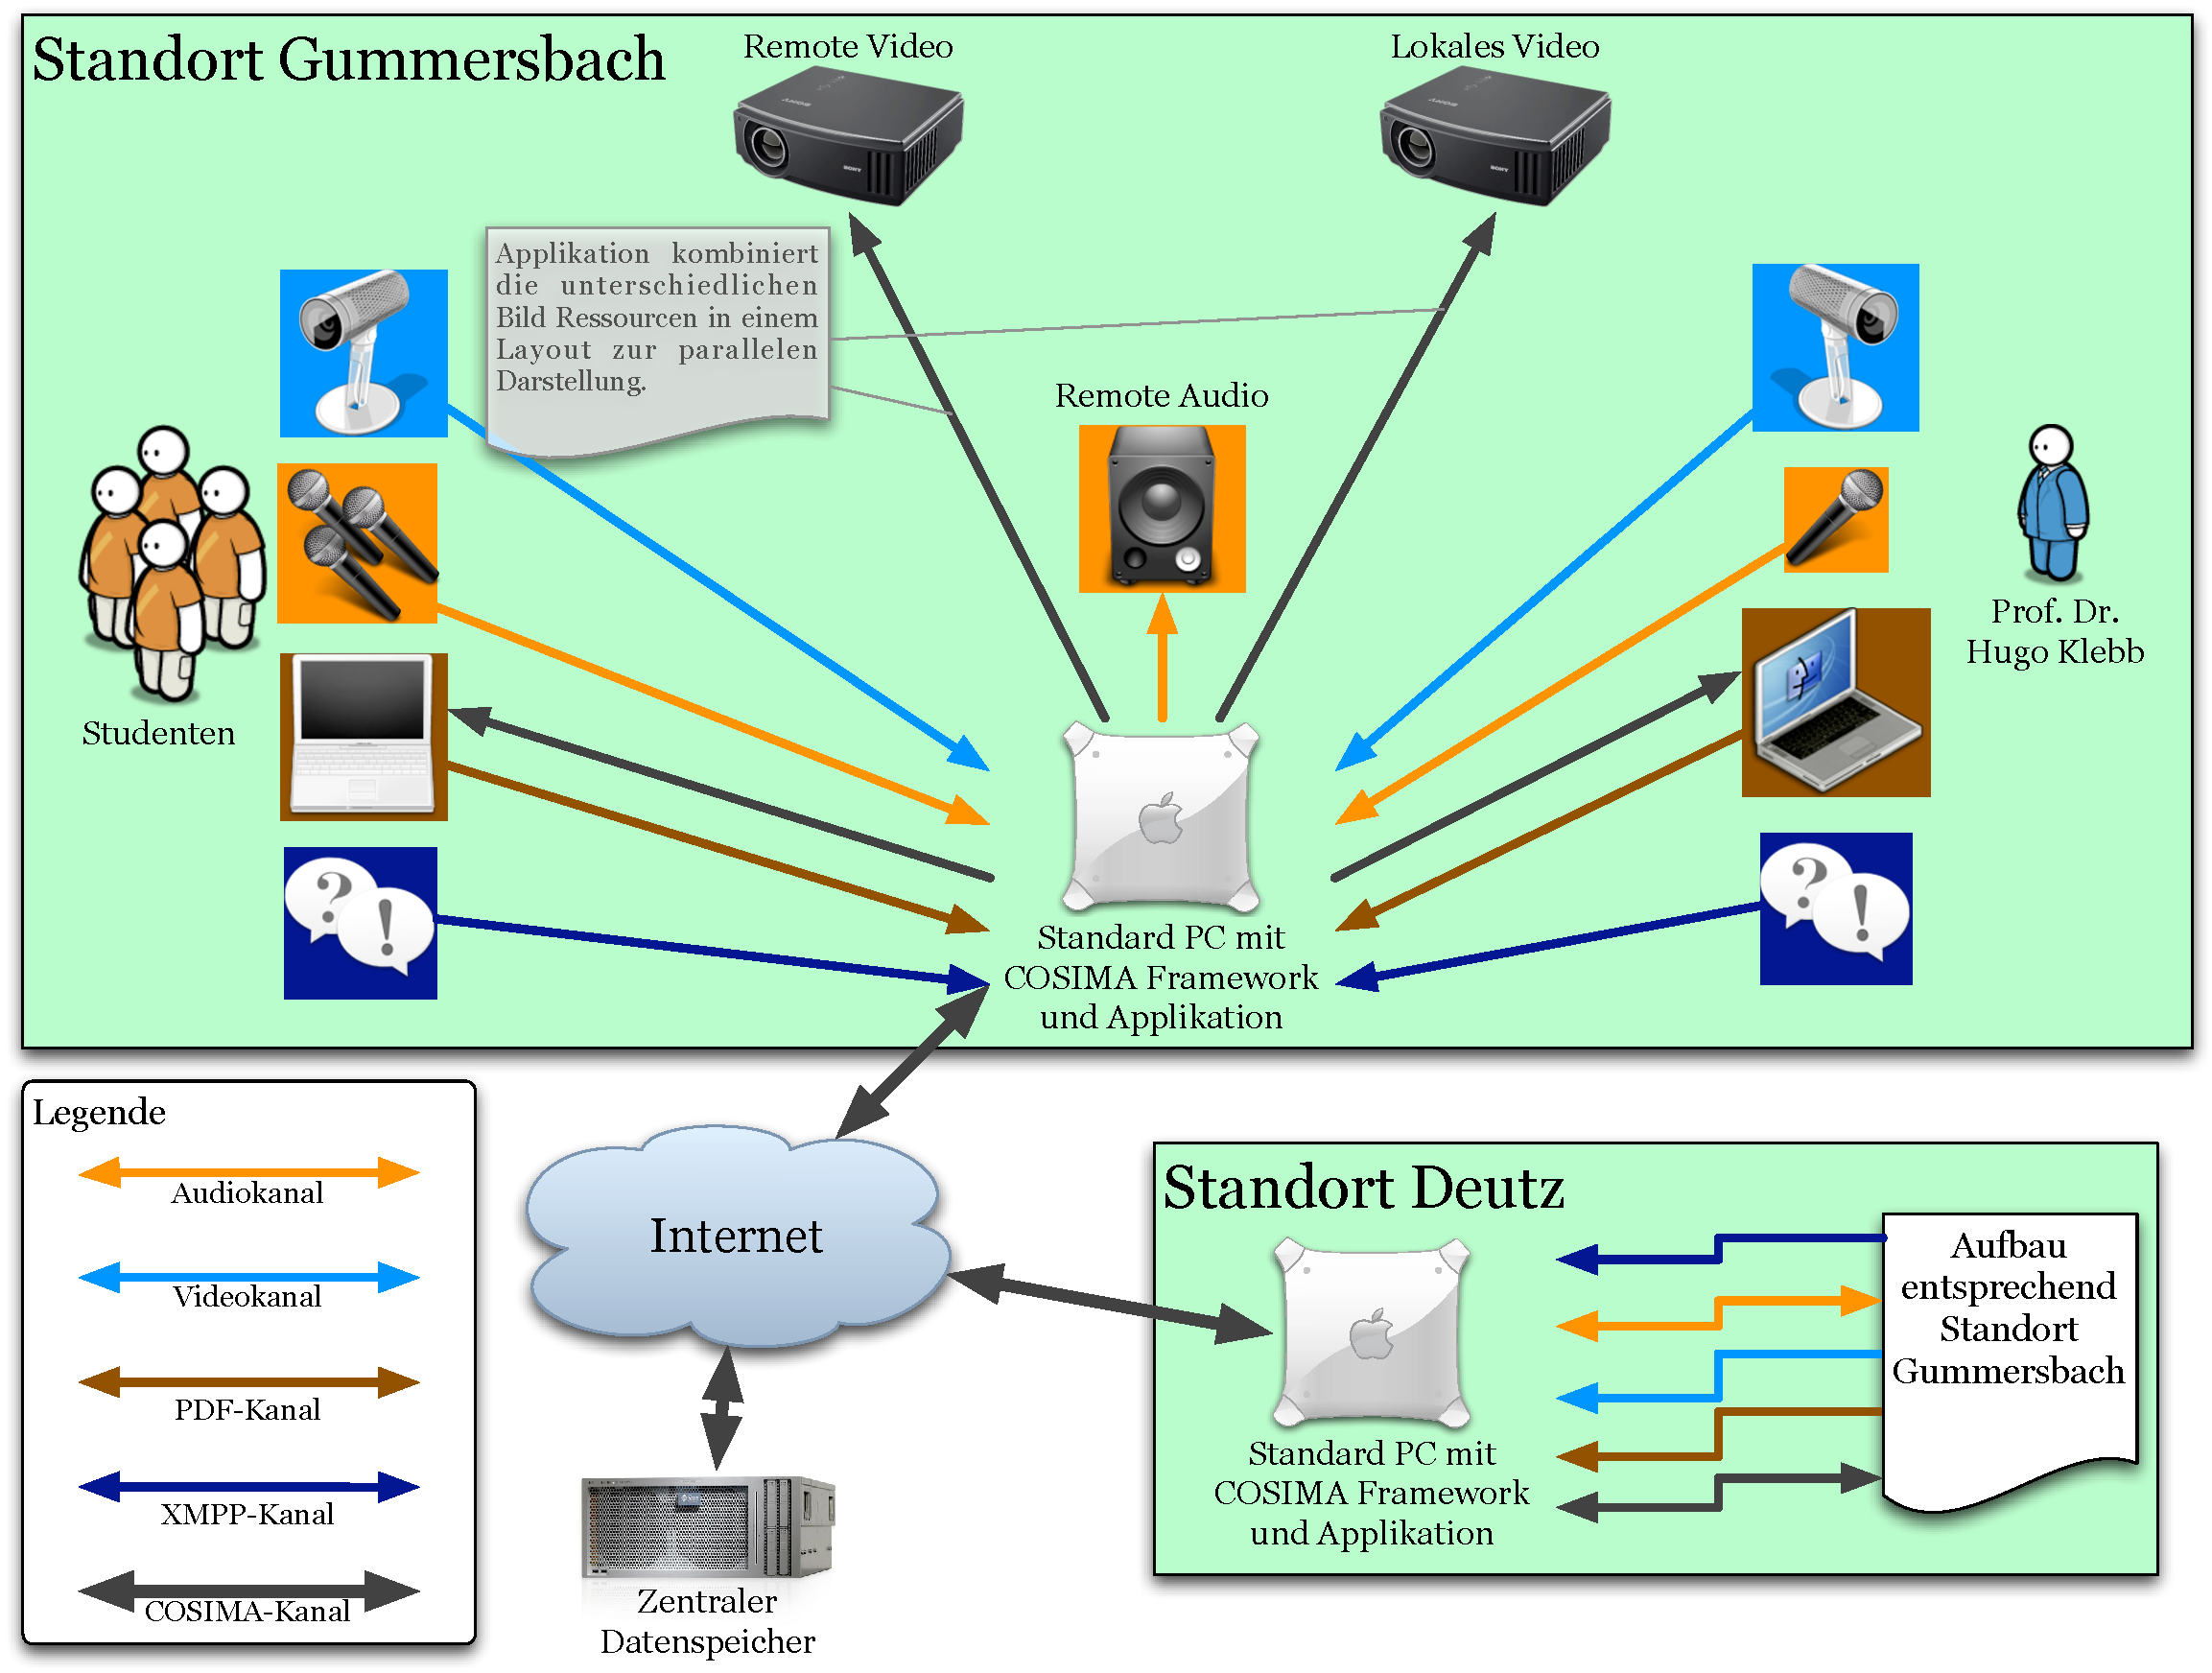
\includegraphics[width=.9\textwidth]{images/Hardware_und_Kanaele.pdf}
  \caption{Diagramm der verwendeten Hardware und Kanäle im Szenario}
  \label{fig:images_Hardware_und_Kanaele}
\end{figure}


% section beschreibung_des_szenario (end)

\section{Ablaufbeschreibung mit Personae} % (fold)
\label{sec:ablaufbeschreibung_mit_personae}

Dozenten:
  
  - Prof. Dr. Julius Largo (Deutz)
  - Prof. Dr. Hugo Klebb (Gummersbach)
  
Studenten:

- Thorsten Sommer
- Vanessa Bergmann
- Katrin Schreiber
- Uwe Gaertner
- Swen Reinhard
- Anna Müller
- Ines Gruenewald
- Nicole Eiffel
- Sara Kaiser
- Alexander Feierabend

- Barbara Fenstermacher
- Marina Beike
- Jennifer Werner
- Christin Koehler
- Dieter Beike

% section ablaufbeschreibung_mit_personae (end)

% chapter szenario (end)